\iffalse
\documentclass[journal,10pt,twocolumn]{article}
\usepackage{graphicx}
\usepackage[margin=0.5in]{geometry}
\usepackage{amsmath}
\usepackage{array}
\usepackage{booktabs}
\usepackage{amssymb}
\title{\textbf{Matrix Assignment}}
\author{lakshmi kamakshi}
\date{September 2022}

\begin{document}

\maketitle
\paragraph{\textit{Problem Statement} -
\fi
Two concentric circles are of radii 5cm and 3cm. Find the length of the chord of the larger circle which touches the smaller circle.
	\begin{figure}[!h]
		\centering
 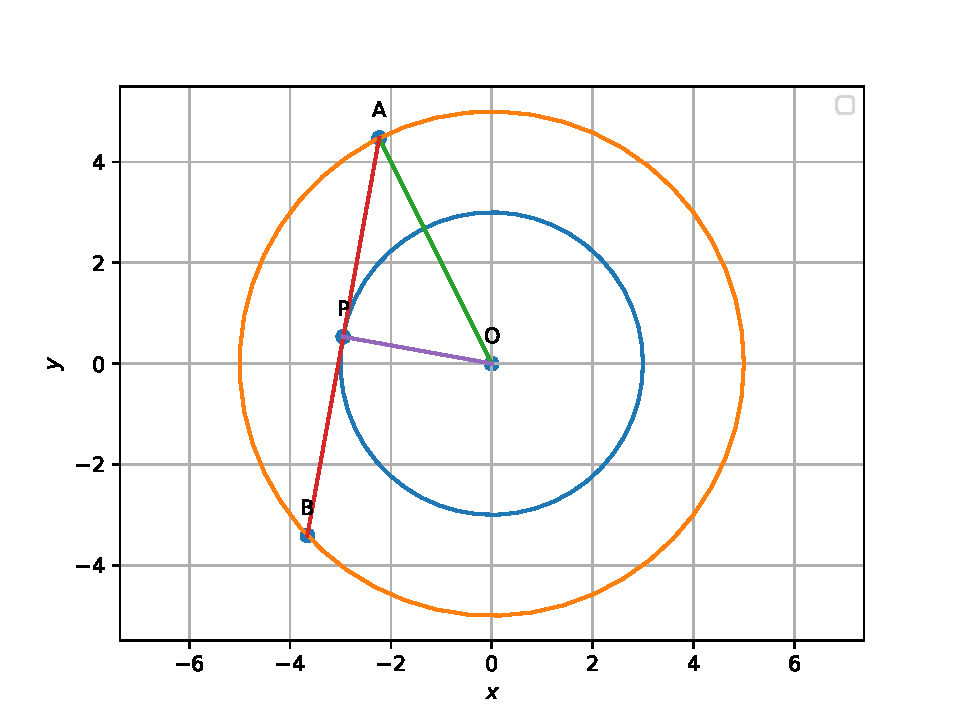
\includegraphics[width=\columnwidth]{chapters/10/10/2/7/figs/fig.pdf}
		\caption{}
		\label{fig:10/10/2/7}
  	\end{figure}
	\\
	\solution  See Fig.
		\ref{fig:10/10/2/7}.  Let 
\begin{align}
	\vec{O} &=
\vec{0}
\\
	r_1 &= 5, r_2 = 3.
\end{align}
Choosing
\begin{align}
	\vec{A} = r_1\myvec{\cos \theta \\ \sin \theta},
\end{align}
$\vec{P}$ can be obtained following the approach in Problem 
\ref{chapters/10/10/2/7}.
From Appendix
	\ref{prop:circ-chord-perp}, $\vec{P}$ is the mid point of $AB$.  This can be used to obtain $\vec{B}$.
\iffalse
\vspace{5mm}

\section*{Solution}

Given the radii of the circles : $3cm$,$5cm$

 r1 = $5cm$ , r2 = $3cm$.
Let,
\begin{eqnarray}
	\boldsymbol{O}-\boldsymbol{A} = \boldsymbol{p}
\\	\boldsymbol{O}-\boldsymbol{P} = \boldsymbol{a}
\\	\boldsymbol{P}-\boldsymbol{A} = \boldsymbol{o}
\end{eqnarray}
\\ From the triangle law of addition of vectors:
\begin{eqnarray}
 \boldsymbol{p} = \boldsymbol{a} + \boldsymbol{o}
\\ \boldsymbol{o} = \boldsymbol{p} - \boldsymbol{a}
\end{eqnarray}
\\ find the magnitude of the vector o 
	\begin{eqnarray}
		||\textbf{o}||^2 = ||\textbf{p-a}||^2
		\\	||\textbf{o}||^2 = |\textbf{p-a}||\textbf{p-a}|^T
		\\||\textbf{o}||^2 = ||\textbf{p}||^2+||\textbf{a}||^2-2\textbf{p.a}^T
		\\ ||\boldsymbol{o}||^2 = \boldsymbol{25 + 9 -2(|\textbf{p}||\textbf{a}|)(cos\theta)}
\end{eqnarray}


\begin{figure}[h]
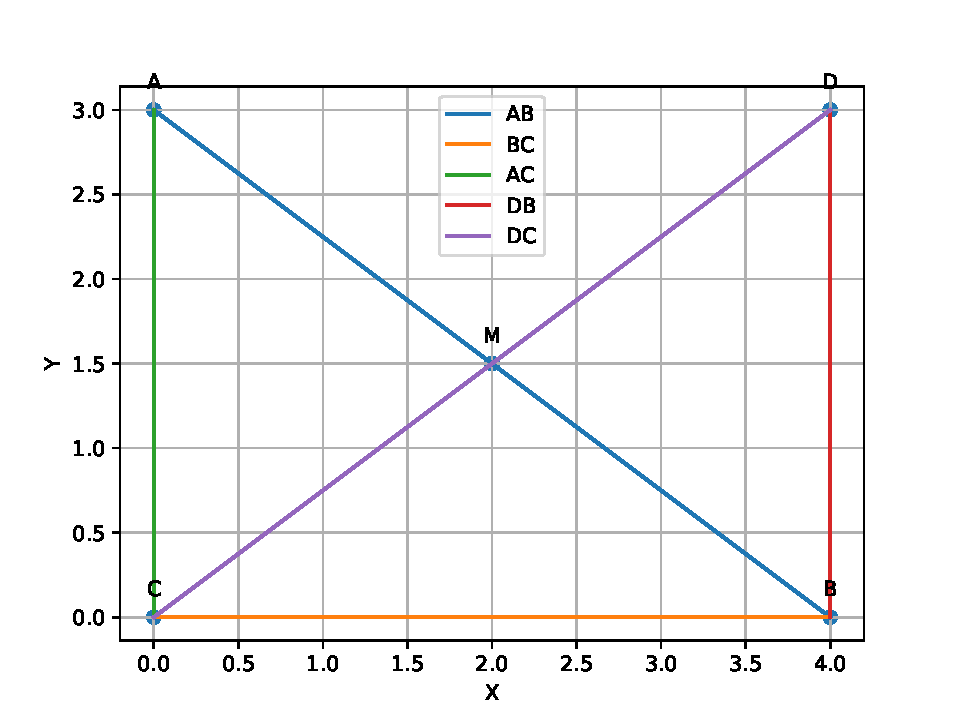
\includegraphics[width=1\columnwidth]{fig.pdf}
\end{figure}
 From the figure, in $\triangle$ OPA:
\begin{equation}
\boldsymbol{cos\theta} = \boldsymbol{\frac{3}{5}}
\end{equation}
\\ Substitute eqn10 value in eqn9
\begin{eqnarray}
||o||^2 = 34 - 2(3)(5)(\frac{3}{5})
\\ ||o||^2 = 34-18
\\ ||o||^2 = 16
\\ \boldsymbol{||o||} =\boldsymbol{4}
\end{eqnarray}
Similarly, in $\triangle$ OPB,
\begin{eqnarray}
	\boldsymbol{P}-\boldsymbol{B} = \boldsymbol{b}
\\	||\boldsymbol{b}|| = 4
\end{eqnarray}
\begin{eqnarray}
	||\boldsymbol{A-B}|| =|\boldsymbol{o}|+|\boldsymbol{b}|
	\\ \boldsymbol{A-B} = 4+4
	\\ \boldsymbol{A-B} = \boldsymbol{8}
\end{eqnarray}
\\ Therefore, the length of the required chord is $8cm$

\section*{Construction}
The input parameters are the lengths $r_1$ and $r_2$ .\\
\setlength \extrarowheight{2pt}
\centering
	\begin{tabular}{|c|c|c|}
	\hline
	\textbf{symbol}&\textbf{value}&\textbf{description}\\
	\hline
	$r_1$&3&OP\\
	\hline
	$r_2$&5&OA\\
	\hline
		$\theta$&acos($\frac{r_1}{r_2}$)&$\angle$O\\
	\hline
	A&$r_1%
	\begin{pmatrix}
		cos(90 -\theta)\\
		sin(90 -\theta)\\
	\end{pmatrix}$%
	&Point A\\
		\hline
	B&$r_1%
		\begin{pmatrix}
			cos(270+\theta)\\
			-sin(270+\theta)\\
		\end{pmatrix}$%
		&Point B\\
	\hline
\end{tabular}
\end{document}
\fi
